\chapter{Demonstration of Baseline Compensation}
\textcolor{red}{基線長補償システムの性能評価をするために、KAAGRAのXアームキャビティを防振した。}

\section{Overview of KAGRA}
\subsection{Status of KAGRA}
KAGRA is a 3km laser interferometer, constructed in Kamioka, Gifu, Japan, and is now in its final commisioning phase. The KAGRA project はこれまでに2つの試験運転を経て、今はLIGOとVirgoとの第三次共同観測(O3)にむけたphaseにいる。Table\ref{tb:tb600}にKAGRAのphaseをまとめる。1つめの試験運転はinitial KAGRA (iKAGRA) と呼ばれる、2016年の3月から4月に行われた、3kmのMichelson interferometerの試験運転である。ことのとき、テストマスは低温ではなく常温ではなかったが、3kmの長期線干渉計を地下で可動させることを実証した。そして次に2つ目の試験運転である、basekine KAGRA (bKAGRA) とよばれる、低温鏡をつかったMicelson干渉計の試験運転である。この運転では低温干渉計を稼働させることを実証した。そして2019年12月現在、LIGOとVirgoとの第三次共同観測(O3)にむけて、低温鏡を使用した Fabry-Perot Michelson interferometer (FPMI)のコミッショニングをおこなっており、中性子連星合体を$1\,\mathrm{Mpc}$で観測できる感度まで向上させるノイズハンティングを行っている。

\begin{table}[h]
  \caption{Summary of the phasec of KAGRA. MI: Michelson Interferometer, FPMI: Fabry-Perot Michelson Interferometer, DRFPMI: Dual-Recycled Fabry-Perot Michelson Interferometer, RSE: resonant sideband extraction}
  \begin{tabular}{lllll}
    \toprule
    &iKAGRA& \begin{tabular}{l}bKAGRA\\Phase1\end{tabular} & \begin{tabular}{l}bKAGRA\\for O3\end{tabular}  & \begin{tabular}{l}bKAGRA\\(final)\end{tabular}  \\ \midrule
        
        \begin{tabular}{l}Year\end{tabular}& \begin{tabular}{l}2016\\Mar - Apr\end{tabular}&\begin{tabular}{l}2018\\Apr - May\end{tabular} & \begin{tabular}{l}2019\\Dec - \end{tabular} & \begin{tabular}{l}2020 -\\(planned)\end{tabular} \\
              \begin{tabular}{l}Configuration\end{tabular} & \begin{tabular}{l}MI\end{tabular} & \begin{tabular}{l}MI\end{tabular} & \begin{tabular}{l}FPMI\end{tabular} & \begin{tabular}{l}DRFPMI\\(RSE)\end{tabular}\\
                      
                      \begin{tabular}{l}Test mass\\temperature\end{tabular} & \begin{tabular}{l}room temp.\end{tabular}& \begin{tabular}{l}18K\\room temp.\end{tabular} & \begin{tabular}{l}18K\\room temp.\end{tabular}  & \begin{tabular}{l}22K\end{tabular}             \\ \bottomrule
  \end{tabular}
\end{table}

%% KAGRAの最終的な感度は、resonant sideband extraction thechnique をもちいた Dual-Recycled Fabry-Perot Michelson interferometer で達成される。KAGRAの設計感度をFig.\ref{img:img600}に示す。

%% \begin{figure}[h]
%%   \begin{center}   
%%     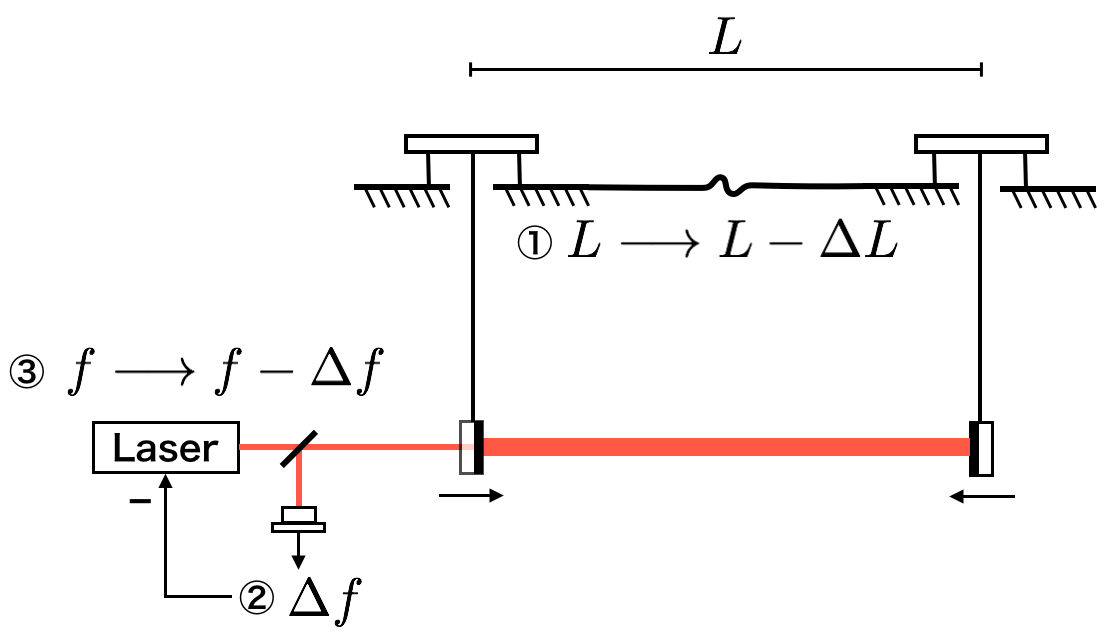
\includegraphics[width=12cm]{./img_chap6/img600.png}
%%     \caption{The designed sensitivity of KAAGRA \cite{akutsu2019first}}{}\label{img:img600}
%%   \end{center}
%% \end{figure}

\subsection{Main Interferometer}
KAGRAのメイン干渉計の図をFig.\ref{img:img601}に示す。KAGRAは他のLIGOやVirgoと同様に、腕にFabry-Perot光共振器とリサイクリング光共振器をもつマイケルソン干渉計である。ただし他とことなるのは、腕共振器の鏡は$22\,\mathrm{K}$まで冷却されていることである。この鏡にはサファイヤを使用している。なぜならば極低温下でも高いthermal conductivity と高いQ値を持ち、それぞれの特徴が熱レンズ効果と熱雑音を低減できるためである。またKAGRAその他の鏡はすべて常温のfused silica 鏡である。

\begin{figure}[p]
  \begin{minipage}{15cm}
    \begin{center}   
      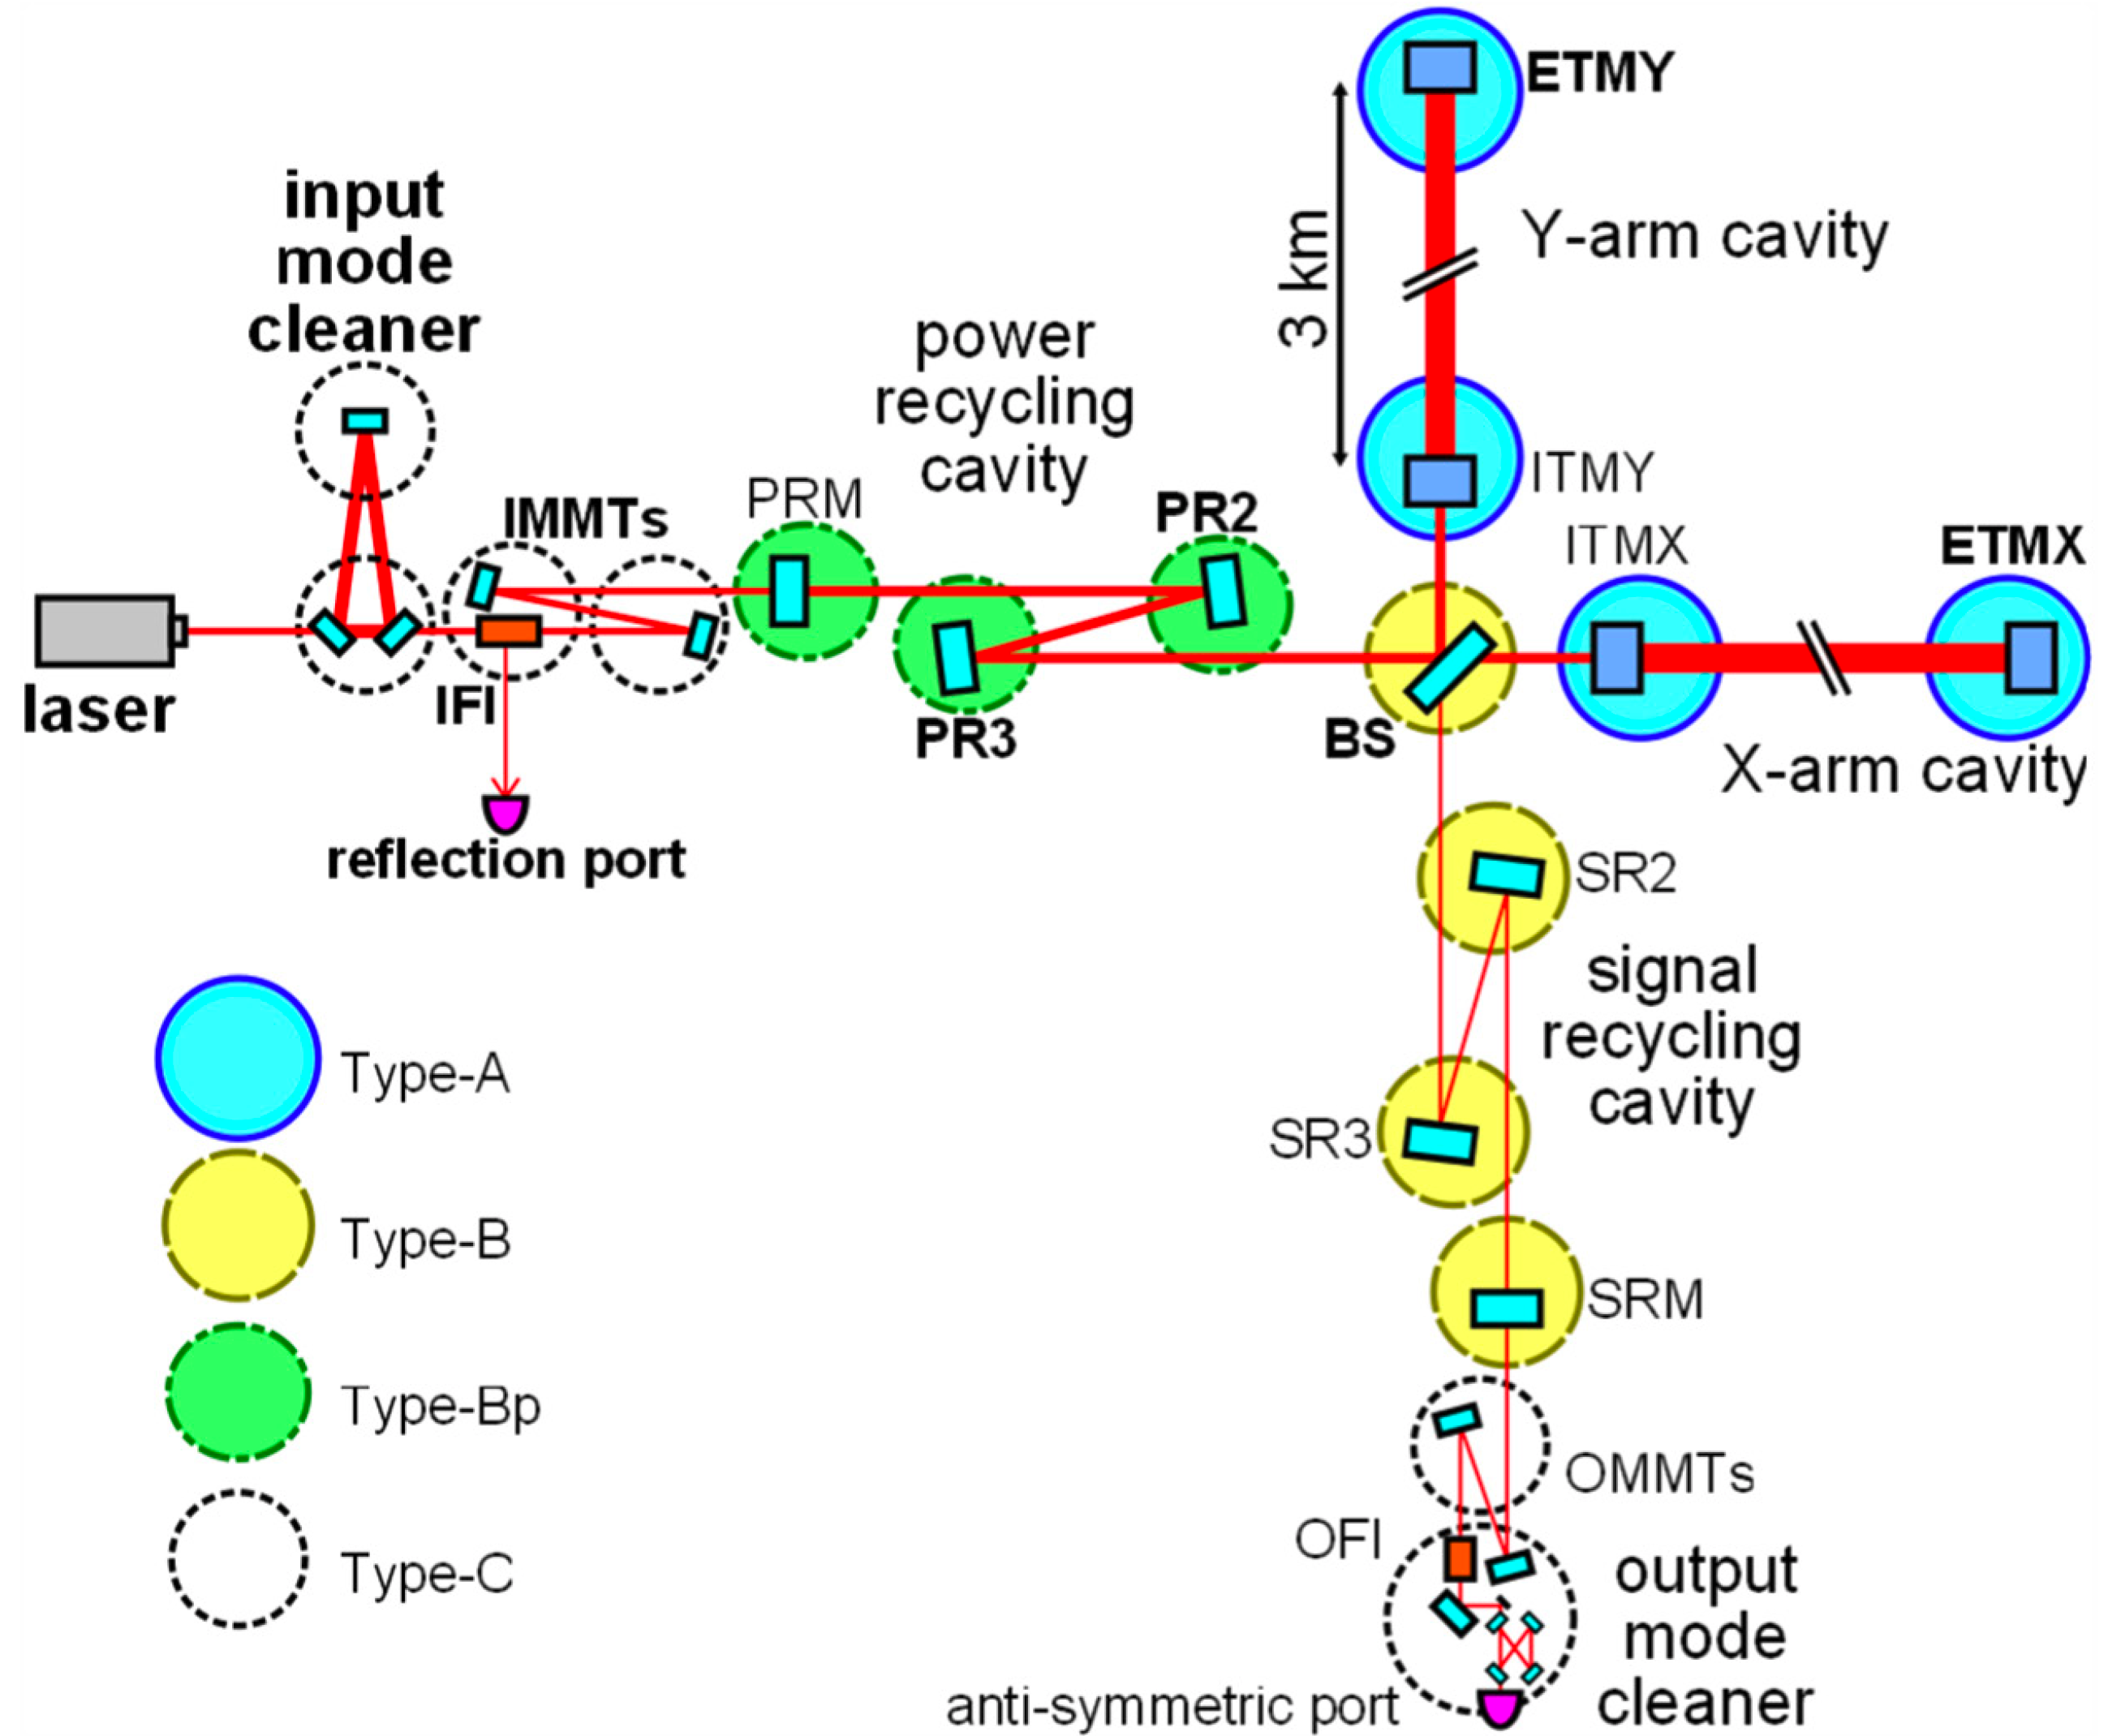
\includegraphics[width=13cm]{./img_chap6/img601.png}
      \subcaption{Schematic interferometer configuration of KAGRA \cite{akutsu2019first}}{}\label{img:img601} \hfill\vspace{10pt}
    \end{center}
  \end{minipage}
  \begin{minipage}{15cm}
    \begin{center}   
      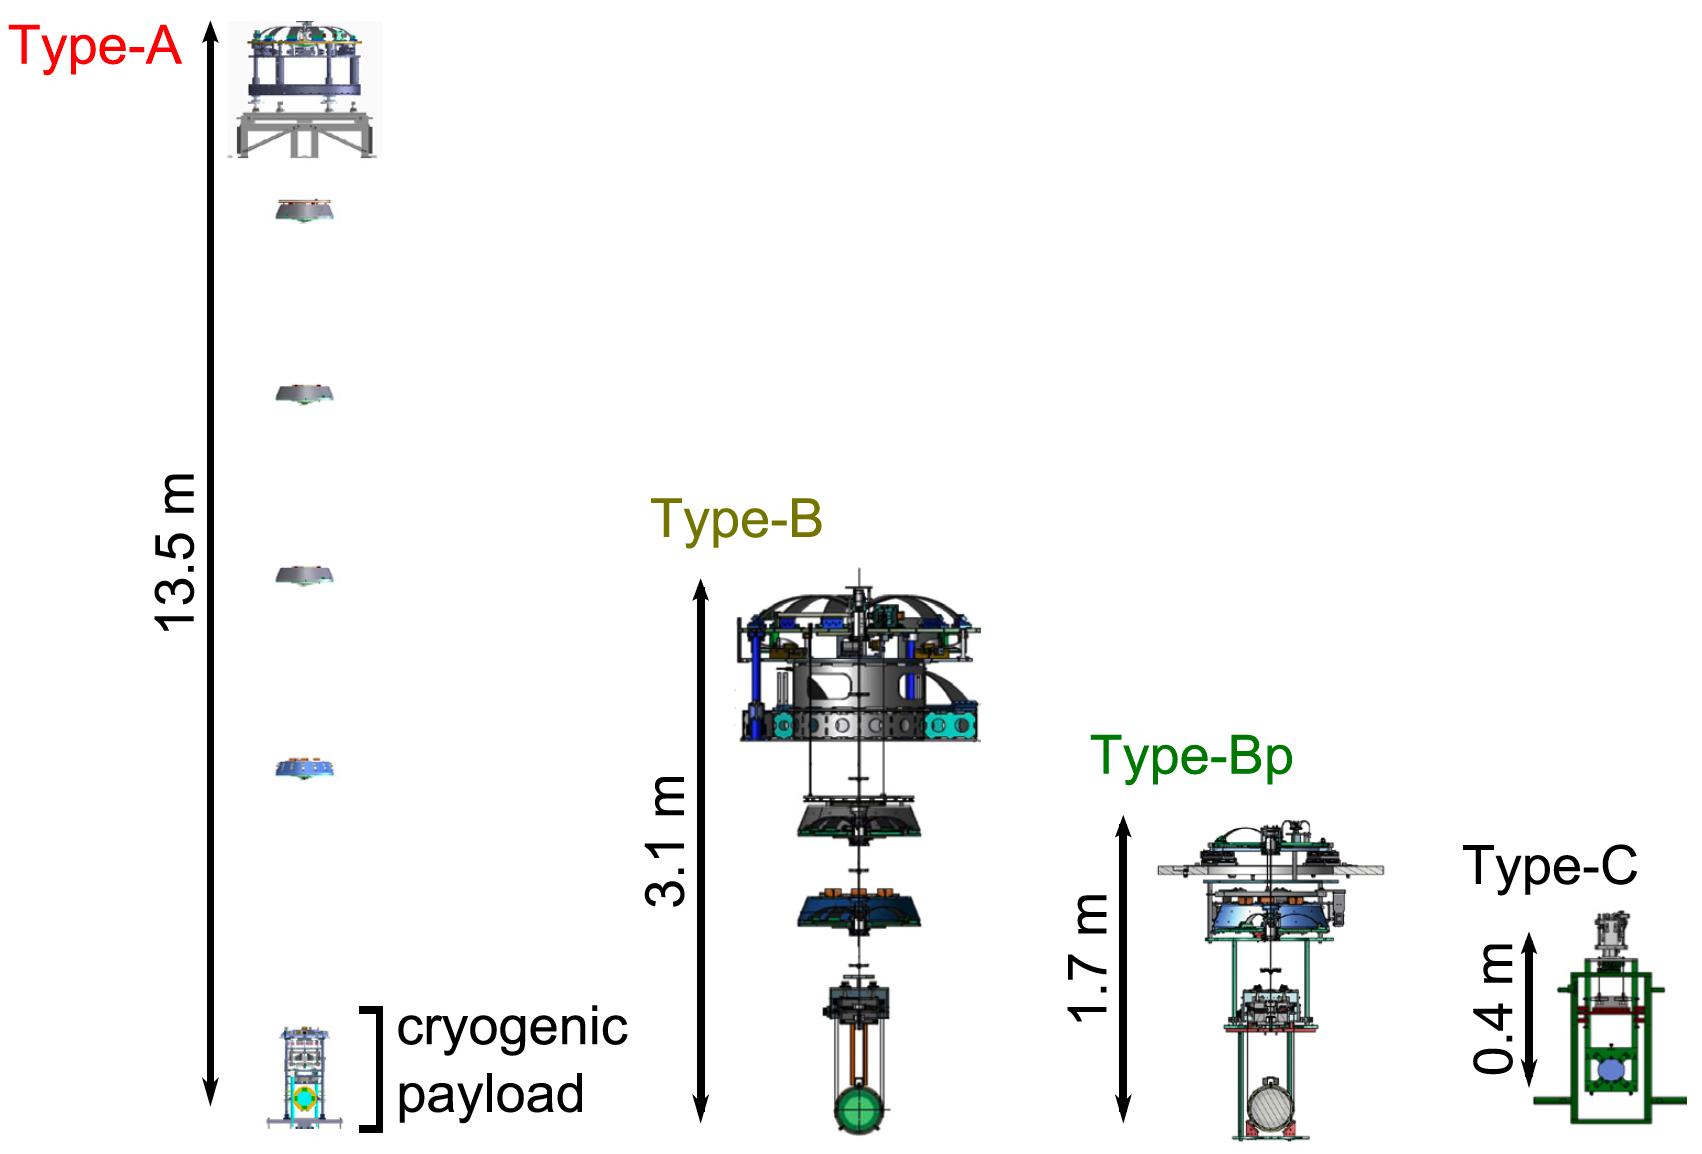
\includegraphics[width=13cm]{./img_chap6/img601b.png}
      \subcaption{KAGRA mirror suspension system \cite{akutsu2019first}}{}\label{img:img601b}
    \end{center}
  \end{minipage}
  \caption{Interferometer configuration and mirror suspension system}{}
\end{figure}


KAGRAの干渉計は、おもに4つに分けられる; arm caivties, input and output mode cleaners (IMC and OMC), power resycling cavities (PRC), and signal resycling cavities (SRC).

Arm cavities are composed of input test masses (ITMs) and end test masses (ETMs). また低温鏡であるITM内部でのパワーをへらすために、フィネスは1530と他の検出器とくらべて高い。

IMCは入射光の空間モードの整形と周波数を安定化させるために使われ、OMCは出射光のunwanted higher-order spatial modes とfrequency sideband を落とすためにある。IMCは3つの鏡で構成される三角共振器であり、およそ1Hz以上の周波数のpre-stabilizationができるように設計されている。またOMCは4つの鏡から構成されるbow-tie cavityである。

PRC はBSと共振器をつくるPRMの他にPR2とPR3鏡で構成される。この共振器で入射光のパワーを10倍増幅させる。

SRCはSRMとSR2、SR3で構成される。SRCは検出器を広帯域にして重力波信号を抜き出すために使われる。This technique is more important than Advanced LIGO and Advanced Virgo, because the bandwidth is narrower than other detectors due to a high finesse arm cavity of KAGRA. 



\subsection{Mirror Suspension System}

\section{KAGRA Type-A Suspension}
\subsection{Overview}

\subsection{Mechanical design}
\subsubsection{Pre-Isolator stage (PI)}

\subsection{Sensors and Actuators}
\subsubsection{Liner Variable Differential Transducer (LVDT)}
\subsubsection{Geophone}
\subsubsection{Coil-magnet actuator}




\section{Experimental Arrangement}
\subsection{X-arm Cavity}
\subsection{...}
\section{Results}
\subsection{...}
\section{Discussion and Summary of the Chapter}
\subsection{Discussion}
\subsection{Summary}
